\documentclass{article}

% Language setting
% Replace `english' with e.g. `spanish' to change the document language
\usepackage[english]{babel}


% Set page size and margins
% Replace `letterpaper' with `a4paper' for UK/EU standard size
\usepackage[a4paper, top=2cm,bottom=2cm,left=3cm,right=3cm,marginparwidth=1.75cm]{geometry}

% Useful packages
\usepackage{amsmath,amsfonts}
\usepackage{graphicx,caption}
\usepackage{authblk}
\usepackage{float}
\usepackage[colorlinks=true, allcolors=blue]{hyperref}
\usepackage{natbib}
\usepackage{indentfirst}
\usepackage{amsmath}
% \usepackage{palatino}

\title{A Mathematical Model for Human Fecundability and Aneuploidy-driven Pregnancy Loss}

\author[1]{Arjun Biddanda}
\author[1]{Sara A. Carioscia}
\author[1]{Rajiv C. McCoy}
\affil[1]{Department of Biology, Johns Hopkins University}

\begin{document}
\maketitle

\section*{Model Description}

In the original model from \citep{Macklon2002-zn}, the ``iceberg'' of pregnancy loss probabilities is framed as the \textit{absolute} probability of the pregnancy loss outcome (\ref{fig:1}). However, in many ways it may be more favorable to model the series of \textit{conditional} probabilities that underlie each section of the iceberg. 

\begin{figure}[H]
\begin{center}
    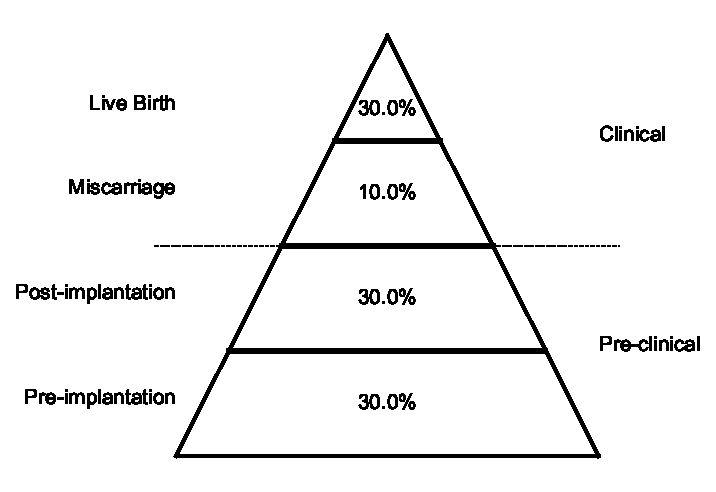
\includegraphics[width=0.5\textwidth]{figures/macklon_recreate.041724.pdf}
\end{center}
\vspace{-1.5em}
\caption{The ``Iceberg'' of pregnancy loss (repurposed from \citep{Macklon2002-zn}).}
\label{fig:1}
\end{figure}

We provide an introduction to the model below, with the conditional probabilities. The  probability we would like to model is the probability of a \textit{live birth conditional on conception occurring}. We model this using a series of conditional probabilities: 

\begin{equation}
	P(\text{Live Birth}) =  (1 - P(\text{Miscarriage} | \text{no EPL})) \cdot (1 - P(\text{EPL} | \text{implantation})) \cdot (1 - P(\text{failed implantation}))
\end{equation}

This model posits that a health live birth (conditional on conception occurring) is conditional on no implantation failure, no early pregnancy loss, \textit{and} no miscarriages.

While there may be a number of potential factors influencing both of these negative events during pregnancy, we primarily focus on the assumption that aneuploidy drives a large fraction of these effects. We first posit that the distribution of aneuploidy outcomes come from the following distribution: 

\begin{equation}
\begin{aligned}
P(\text{Aneuploidy} = a) &= \begin{cases}
0.5 &, a = \text{Euploid}\\
0.25 &, a = \text{Meiotic}\\
0.25 &, a = \text{Mitotic}\\
\end{cases}
\end{aligned}
\end{equation}

These are approximate, but as long as $1 = \sum_{a \in \mathcal{A}} P(\text{Aneuploidy} = a)$, all of the following aspects of the model follow. 

\subsubsection*{Implantation Failure}

The second conditional model is the implantation failure rate: 

\begin{equation}
P(\text{failed implantation} | \text{Aneuploidy}) = \begin{cases}
0.16 &, a = \text{Euploid}\\
0.36 &, a = \text{Meiotic}\\
0.57 &, a = \text{Mitotic}\\
\end{cases}
\end{equation}

This conditional probability suggests that different forms of aneuploidy have different impacts on implantation - roughly corresponding to when they arise during development (e.g. meiotic-origin being the earliest). We have approximated the rate of implantation failure here as the probability of embryo arrest from \citep{McCoy2023-dg} (Figure 3B) -- however there may be other reasons beyond aneuploidy for implantation to fail.  

We can then calculate the following absolute probability:

\begin{equation}
P(\text{failed implantation}) = \sum_{a} P(\text{failed implantation} | \text{Aneuploidy} = a) P(\text{Aneuploidy} = a) ,
\end{equation}

which directly corresponds to the bottom section of the iceberg in \citep{Macklon2002-zn}, but importantly now incorporates embryonic aneuploidy. 

% NOTE: we can have this potentially depend on the potential for the implantation checkpoint as well...

\subsubsection*{Early Pregnancy Loss}

We now turn to the second relevant conditional probability for early pregnancy loss (EPL) which is when there is pregnancy loss following a successful implantation but prior to being a clinically-defined miscarriage. 

\begin{equation}
	P(EPL | \text{implantation}, \text{Aneuploidy}=a) = \begin{cases}
	\epsilon &, a= \text{Euploid}\\
	1 - \eta &, a = \text{Meiotic}\\
	1 - \eta &, a = \text{Mitotic}\\
	\end{cases},
\end{equation}

where $\eta$ is an "escape" probability where a meiotic or mitotic aneuploidy does not lead to early-pregnancy loss and $\epsilon$ is the probability lethal genetic mutations that may lead to aberrant pregnancy outcomes even within a euploid embryo \footnote{The parameter $\epsilon$ can also represent the probability of smaller scale, but still lethal, structural variants so can be thought of as a larger catch-all for lethal mutations that survive implantation but still lead to inviability}. 

The corresponding absolute probability for this section of the ``iceberg'' is: 

\begin{equation}
\begin{aligned}
P(EPL) &= \sum_{a} P(EPL | \text{implantation}, \text{Aneuploidy}=a) \\
&\cdot (1 - P(\text{failed implantation} | \text{Aneuploidy} = a))\\ 
&\cdot P(\text{Aneuploidy} = a)
\end{aligned}
\end{equation}

\subsubsection*{Miscarriage}

The final consideration is the conditional probability of a miscarriage, conditional on surviving beyond EPL and implantation. 

\begin{equation}
	P(Miscarriage | \text{Aneuploidy}=a) = \begin{cases}
	0.3 &, a= \text{Euploid}\\
	0.3 &, a = \text{Meiotic}\\
	0.3 &, a = \text{Mitotic}\\
	\end{cases},
\end{equation}


In most cases however, we do not have strong estimates for whether the miscarriage was the result of an aneuploidy or not. However, in almost all birth cohort datasets the occurrence of miscarriages reflects a strong U-shaped trend  with maternal age \citep{Gruhn2019-al}. 

% NOTE: look at BGI 

\subsubsection*{Accounting for Maternal Age} 

Since maternal age has a well-documented effect on aneuploidy abundance ... 

\textbf{NOTE: here we will use the inferred function from Gruhn et al for the probability of meiotic aneuploidy as a function of age}



\section*{Results}

% NOTE: small figure on extending this to different ages?



\bibliographystyle{plainnat}
\bibliography{refs}

\end{document}
